\documentclass[border=5pt]{standalone}
\usepackage{tikz-cd,pgfplots}
\pgfplotsset{compat=1.14}
\begin{document}
\begin{tabular}{cc}
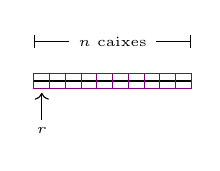
\begin{tikzpicture}[scale=1]
\draw[|-|,thin] (-2,1.5) -- node[midway,fill=white] {\tiny{$n$ caixes}} (0,1.5);
\draw[thin] (-2,1) -- (0,1);
\draw[thin,violet] (-2,1.1) -- (0,1.1);
\draw[thin,violet] (-2,0.9) -- (0,0.9);
\foreach \x in {-2,-1.8,...,0}{
 \draw[thin,violet](\x,0.9)--(\x,1.1);}
\node (a) at (-1.9,0.375) {\tiny{$r$}};
\draw[thin,->] (-1.9,0.5)--(-1.9,0.85);
%\draw (-2,1) -- (-1.8,1) node[midway,yshift=-1em]{$r=1/n$};
%\draw[thin,violet] (5/10,1/10) -- (7/10,1/10);
%\draw[thin,violet] (5/10,-1/10) -- (7/10,-1/10);
%\foreach \x in {5/10,7/10}{
% \draw[thin,violet](\x,-1/10)--(\x,1/10);}
%\node[above] (a) at (-1/10,1/10) {$\frac{1}{n}$};  
\end{tikzpicture}
%\begin{tikzpicture}[scale=0.1]
%\draw[thin,violet] (-2,1) -- (0,1);
%\draw[thin,violet] (-2,-1) -- (0,-1);
%\foreach \x in {-2,0}{
% \draw[thin,violet](\x,-1)--(\x,1);}
%\node[above] (a) at (-1,1) {$\frac{1}{n}$}; 
%\end{tikzpicture}
&
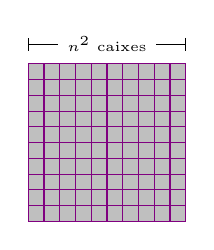
\begin{tikzpicture}[scale=1]
\fill[lightgray] (-2,0)--(0,0)--(0,2)--(-2,2);
\foreach \x in {0,0.2,...,2}{
\draw[thin,violet] (-2,\x) -- (0,\x);
}
\foreach \x in {-2,-1.8,...,0}{
\draw[thin,violet] (\x,0) -- (\x,2);
}
\draw[|-|,thin] (-2,2.25) -- node[midway,fill=white] {\tiny{$n^2$ caixes}} (0,2.25);
\end{tikzpicture} 
%\begin{tikzpicture}[scale=0.1]
%\foreach \x in {0,2}{
%\draw[thin,violet] (-2,\x) -- (0,\x);
%}
%\foreach \x in {-2,0}{
%\draw[thin,violet] (\x,0) -- (\x,2);
%}
%\node[above] (a) at (-1,1.75) {$\frac{1}{n}$}; 
%\end{tikzpicture}
\\
\\
\multicolumn{2}{c}{
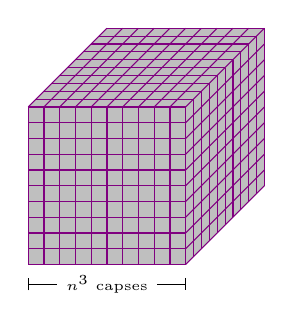
\begin{tikzpicture}[scale=1]
%front side
\fill[lightgray] (-2,0)--(0,0)--(0,2)--(-2,2);
\fill[lightgray] (0,0)--(1,1)--(1,3)--(0,2);
\fill[lightgray] (-2,2)--(0,2)--(1,3)--(-1,3);
\foreach \x in {0,0.2,...,2}{
\draw[thin,violet] (-2,\x) -- (0,\x);
}
\foreach \x in {-2,-1.8,...,0}{
\draw[thin,violet] (\x,0) -- (\x,2);
}
% right side
\foreach \x in {0,0.2,...,2}{
\draw[thin,violet] (0,\x) -- (1,\x + 1);
}
\foreach \x in {0.1,0.2,...,1}{
\draw[thin,violet] (\x,\x) -- (\x,\x +2);
}
%top side
\foreach \x in {-2,-1.8,...,-0.2}{
\draw[thin,violet] (\x,2) -- (\x+1,3);
}
\foreach \x in {2.1,2.2,...,3}{
\draw[thin,violet] (\x-4,\x) -- (\x-2,\x);
}
\draw[|-|,thin] (-2,-0.25) -- node[midway,fill=white] {\tiny{$n^3$ capses}} (0,-0.25);
\end{tikzpicture}}

%\begin{tikzpicture}[scale=.1]
%%front side
%\foreach \x in {0,2}{
%\draw[thin,violet] (-2,\x) -- (0,\x);
%}
%\foreach \x in {-2,0}{
%\draw[thin,violet] (\x,0) -- (\x,2);
%}
%% right side
%\foreach \x in {0,2}{
%\draw[thin,violet] (0,\x) -- (1,\x + 1);
%}
%\foreach \x in {0,1}{
%\draw[thin,violet] (\x,\x) -- (\x,\x +2);
%}
%%top side
%\foreach \x in {-2,-0}{
%\draw[thin,violet] (\x,2) -- (\x+1,3);
%}
%\foreach \x in {2,3}{
%\draw[thin,violet] (\x-4,\x) -- (\x-2,\x);
%}
%\node[above] (a) at (-.5,2.5) {$\frac{1}{n}$}; 
%\end{tikzpicture}
\end{tabular}
\end{document}
